%!TEX encoding = UTF-8 Unicode
%!TEX root = ../compendium2.tex

\Lab{\LabWeekTEN}

\begin{Goals}
\item Kunna skapa och använda matriser.
\item Kunna iterera över matriser med nästlade for-loopar.
\item Kunna använda arv.
\item Träna på att konstruera algoritmer.
\end{Goals}

\begin{Preparations}
\item Gör övning {\tt \ExeWeekTEN} i kapitel \ref{chapter:W10}.

\item Läs igenom hela laborationen och studera den befintliga koden i \code{workspace}.

\item Skriv pseudokod för metoderna \code{draw} och {walk}, som beskrivs nedan.
\end{Preparations}

\subsection{Bakgrund}

En labyrint är ett rum som har en ingång och en utgång.  I denna laboration ska du rita labyrinter och sedan implementera en algoritm för att hitta ut ur labyrinter.

För våra labyrinter gäller följande begränsningar: Ingången är alltid längst ner i labyrinten, och utgången alltid högst upp. Dessutom är alla väggar parallella med antingen x-axeln eller y-axeln.

Man kan representera en sådan labyrint med hjälp av en booelsk matris, så som visas i figur \ref{maze:figboolmatrix}. Varje element i matrisen motsvarar en ruta i labyrinten. Värdet \code{true} i matrisen representerar att det finns en vägg på motsvarande ruta i labyrinten och \code{false} representerar en öppen ruta där man kan gå.

\begin{figure}[h]
	\begin{center}
		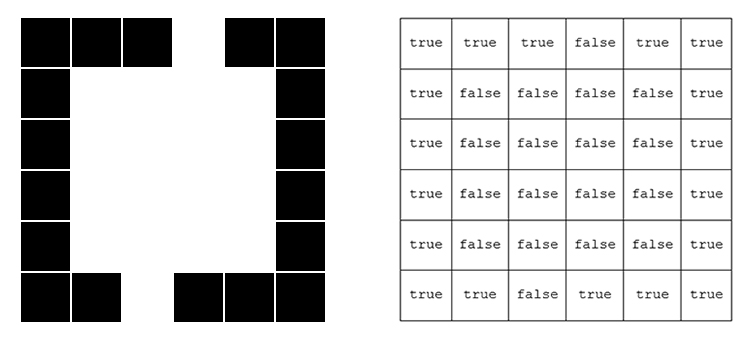
\includegraphics[width=0.7\textwidth]{../img/w09-lab/MazeAndMatrix.jpg}
	\end{center}
	\caption{Exempel på en matrisrepresentation av en enkel labyrint.}
	\label{maze:figboolmatrix}
\end{figure}

Det finns många olika sätt att ta sig igenom en labyrint.\footnote{Om du är intresserad, läs om olika algoritmer för att ta sig igenom en labyrint här: \url{https://en.wikipedia.org/wiki/Maze\_solving\_algorithm}} Ett enkelt sätt att hitta utgången, som kanske inte följer närmsta vägen, är att hålla vänster hand i vänster vägg och följa väggen med handen tills man når öppningen. Detta fungerar för alla labyrinter där väggarna från ingången till utgången är sammankopplade.

När man går igenom labyrinten finns det fyra olika riktningar att välja mellan som alla kan beskrivas i antal grader räknat från x-axeln, där höger motsvaras av 0 grader, uppåt motsvaras av 90 grader, vänster av 180 grader och nedåt av 270 grader.

I denna laboration ska du använda den nästan färdiga case-klassen \code{Maze} som representerar en labyrint med hjälp av en booelsk matris implementerad som en \code{Vector[Vector[Boolean]]}. Du ska implementera metoden \code{draw} som ritar ut matrisen i ett fönster. I den frivilliga extrauppgiften implementerar du metoden \code{random} i kompanjonsobjektet \code{Maze} som ska generera slumplabyrinter.


Klassen \code{Maze} har följande specifikation:

\begin{ScalaSpec}{Maze}
/**
 *  A class representing a maze.
 */
case class Maze(data: Vector[Vector[Boolean]]) {

  /**
   *  Returns a corresponding char from a boolean.
   *  @param b	The boolean which to convert to a char
   */
  def boolToChar(b: Boolean): Char

  /**
   *  Returns a String representation of the maze.
   */
  override def toString: Unit

  /**
   *  Checks if the coordinates x, y is inside the maze and if
   so returns true, otherwise false.
   *  @param x		The x coordinate
   *  @param y		The y coordinate
   */
  private def insideMaze(x: Int, y: Int): Boolean

  /**
   *  Returns the x coordinate of the entry of the maze.
   */
  def getXEntry(): Int

  /**
   * Returns the y coordinate of the entry of the maze.
   */
  def getYEntry(): Int

  /**
   *  Checks if there is a wall left of the coordinates x, y at
   given direction and if so returns true, otherwise false.
   *  @param direction	The direction of the turtle
   *  @param x					The x coordinate
   *  @param y					The y coordinate
   */
  def wallAtLeft(direction: Int, x: Int, y: Int): Boolean

  /**
   *  Checks if there is a wall in front of the coordinates x, y at
   given direction and if so returns true, otherwise false.
   *  @param direction	The direction of the turtle
   *  @param x					The x coordinate
   *  @param y					The y coordinate
   */
  def wallInFront(direction: Int, x: Int, y: Int): Boolean

  /**
   *  Checks it the coordinates x, y is at the exit of the maze.
   *  @param x					The x coordinate
   *  @param y					The y coordinate
   */
  def atExit(x: Int, y: Int): Boolean

  /**
   *  Goes through the the maze and for every spot that is a wall
   draws a brick of size blockSize in SimpleWindow.
   *  @param w		The window in which to draw the maze
   */
  def draw(w: SimpleWindow): Unit = ???
}

/**
 *  A companion object with factory methods for creating maze instances.
 */
object Maze {

  /**
   *  Returns a Maze from a vector of Strings.
   *  @param xs	The vector of Strings that represent the maze
   */
  def fromStrings(xs: Vector[String]): Maze

  /**
   *  Returns a Maze from a specified file.
   *  @param fileName	   The name of the file that represent the maze
   */
  def fromFile(fileName: String): Maze

  /**
   *  Returns a Maze from a sequence of Strings.
   *  @param rows	The sequence of Strings that represent the maze
   */
  def apply(rows: String*): Maze

  /**
   *  Creates and returns a random maze.
   *  @param rows		The number of rows for the maze
   *  @param cols		The number of columns for the maze
   */
  def random(rows: Int, cols: Int): Maze = ???
}

\end{ScalaSpec}


\subsection{Obligatoriska uppgifter}

I de obligatoriska uppgifterna ska du implementera följande:
\begin{itemize}
\item Metoden \code{draw} i klassen \code{Maze}.

\item Klassen \code{MazeTurtle} enligt specifikation nedan och dess metod \code{walk}, som ritar ut var sköldpaddan går medan den finner vägen ut ur en labyrint. \code{MazeTurtle} ska vara en subtyp till befintliga \code{ColorTurtle} som i sin tur är en subtyp till befintliga \code{Turtle}.

\end{itemize}


\noindent Innan du börjar med uppgifterna nedan, studera noga dessa givna filer:
\begin{itemize}
\item
\href{https://github.com/lunduniversity/introprog/tree/master/workspace/w09_maze/src/main/scala/maze/Maze.scala}{workspace/w09\_maze/src/main/scala/maze/Maze.scala} \\
Kompanjonsobjektet \texttt{Maze} innehåller fabriksmetoder som skapar nya labyrintinstanser. Fabriksmetoderna  skapar booelska matriser utifrån strängar, där tecknet '\#' i en sträng representerar en väggruta medan blanksteg representerar en gångruta.

\item
\href{https://github.com/lunduniversity/introprog/tree/master/workspace/w09_maze/src/main/scala/maze/Turtle.scala}{workspace/w09\_maze/src/main/scala/maze/Turtle.scala}

\item
\href{https://github.com/lunduniversity/introprog/tree/master/workspace/w09_maze/src/main/scala/maze/ColorTurtle.scala}{workspace/w09\_maze/src/main/scala/maze/ColorTurtle.scala}

\item Huvudprogrammet \code{main} finns i filen \code{AMazeIngRace.scala}:\\
\href{https://github.com/lunduniversity/introprog/tree/master/workspace/w09_maze/src/main/scala/maze/AMazeIngRace.scala}{workspace/w09\_maze/src/main/scala/maze/AMazeIngRace.scala}

\item Labyrinterna i mappen \code{resources}:\\
\href{https://github.com/lunduniversity/introprog/tree/master/workspace/w09_maze/src/main/resources}{workspace/w09\_maze/src/main/resources}

\end{itemize}

\Task Kör igång huvudprogrammet i filen \code{AMazeIngRace.scala} och säkerställ att ditt projekt hittar \code{SimpleWindow} i \code{cslib}, samt att labyrintfilerna i mappen \code{src/resources} hittas av huvudprogrammet och skrivs ut.

\Task Implementera metoden \code{draw} i klassen \code{Maze} så att den ritar upp en labyrint i \texttt{SimpleWindow}, enligt nedan tips:

\begin{itemize}
\item Du behöver gå igenom matrisen \texttt{data} och undersöka elementen på varje plats. Om elementet på en viss plats är \texttt{true} ska det ritas upp en bit av en vägg på motsvarande plats i \texttt{SimpleWindow}.
Till din hjälp har du den färdigskrivna metoden \texttt{brickInTheWall}.

\item Om elementet på en viss plats är \texttt{false} ska ingenting ritas upp.

\item Börja, som förberedelse, att skissa på pseudokod för uppgiften. Du använder lämpligen en nästlad for-sats.

\item En speciell utmaning är att förstå skillnaden mellan fönstrets koordinater och positionen i den booelska labyrintmatrisen, samt hur översättningen mellan dessa går till. Rita gärna en skiss med exempel på papper för att reda ut detta.
\end{itemize}


\Task Skapa din egen labyrint i en textfil kallad \texttt{maze5.txt} i mappen \code{resources}. Kontrollera så att även denna labyrint ritas upp som den ska, och fixa annars till metoden \texttt{draw} så att den fungerar som tänkt. Din labyrint behöver inte alls vara avancerad; det är inte meningen att den här uppgiften ska ta lång tid.


\Task I denna uppgift ska du implementera en algoritm som får en sköldpadda att ta sig genom en labyrint. Algoritmen ska baseras på idén att alltid hålla vänster hand i väggen (eller sköldpaddsfot i det här fallet). För detta ändamål ska du skapa en ny klass \texttt{MazeTurtle} enligt följande specifikation:

\begin{ScalaSpec}{MazeTurtle}
/**
  * A Turtle that can walk through a maze with a specified color.
  *
  * @param window The window the turtle should be placed in.
  * @param maze   The maze in which the turtle will walk.
  * @param color  The color with which the turtle will walk.
  */
class MazeTurtle(window: SimpleWindow,
                 maze: Maze,
                 color: Color)
  extends ColorTurtle(
    window,
    initPosition = Point(maze.getXEntry, maze.getYEntry),
    initColor = color
  ) {

  /**
    * Lets the turtle walk through the maze from entry to exit by
    * following the wall to left side of the turtle.
    */
  def walk(): Unit = ???

}

\end{ScalaSpec}

\begin{itemize}
\item Klassen \texttt{MazeTurtle} ska ärva klassen \texttt{ColorTurtle} och ha en extra parameter, nämligen den labyrint som sköldpaddan ska gå i.

\item Börja, som förberedelse, att skriva pseudokod för algoritmen, enligt tipsen i följande punkter.

\item Implementera metoden \texttt{walk} i \texttt{MazeTurtle}, med hjälp av tekniken att alltid hålla vänster extremitet i väggen, så att sköldpaddan tar sig genom labyrinten från början till slut. Varje steg motsvarar att flytta sig från en ruta till en annan i \code{Boolean}-matrisen i \texttt{Maze}.

\item Sköldpaddan kommer alltså att ta sig fram i labyrinten genom att undersöka för varje steg om den borde svänga vänster, gå rakt fram eller svänga höger, beroende på hur den står i förhållande till vänster vägg.

\item För att avgöra hur sköldpaddan ska gå, ska du använda dig av metoderna \texttt{wallInFront} och \texttt{wallAtLeft} som finns färdiga i \texttt{Maze}.

\item Använd gärna en fördröjning i din algoritm, t.ex. \code{SimpleWindow.delay(20)}, så att du hinner begrunda hur din labyrintsköldpadda går i labyrinten. Men för stora labyrinter är det lämpligare med \code{SimpleWindow.delay(1)} för snabbare upprepad testning.

\item Om din algoritm visar sig ha buggar, använd \code{println} för att instrumentera din kod, enligt tipsen som ges i appendix \ref{appendix:debug}.

\end{itemize}

\clearpage

\subsection{Frivillig extrauppgift}

I denna frivilliga extrauppgift ska du generera en slumpmässig labyrint. Du ska använda en förenklad variant av Prims algoritm.\footnote{Om du vill, läs mer om Prims algoritm här: \href{https://en.wikipedia.org/wiki/Prim\%27s_algorithm}{en.wikipedia.org/wiki/Prim\%27s\_algorithm}}

I pseudokoden för vår algoritm, som återfinns nedan, kallas en ruta som inte är en vägg för en \emph{öppen ruta}. Att \emph{öppna en ruta} innebär att en ruta görs om från en vägg till en öppen ruta (om den inte redan är öppen).

Eftersom det i vårt fall endast ska finnas en enda ingång och en enda utgång i labyrinten, måste detta hanteras speciellt.

Först följer en översiktlig beskrivning av algoritmen, sedan pseudokod med mer detaljer.

\begin{enumerate}[noitemsep]
    \item Skapa en matris helt fylld med väggar.
	\item Börja med att slumpmässigt välja en av rutorna i nedersta raden och öppna den rutan, samt rutan ovanför. Detta blir ingången till labyrinten.
	\item Applicera väggöppningsalgoritmen som visualiseras i figur \ref{lab:maze:prims-algo-viz} på sida \pageref{lab:maze:prims-algo-viz}. Observera att matrisens ytterkantsväggar inte ska öppnas (förutom ingången och utgången).
	\item Slutligen letar vi efter en slumpmässig ruta på näst översta raden som är öppen och öppnar rutan ovanför denna, vilket blir utgången.
\end{enumerate}

\begin{CodeSmall}
  def random(rows: Int, cols: Int): Maze = {
    val maze: Array[Array[Boolean]] = /*initialt en matris med bara väggar*/
    val wallCandidates: ArrayBuffer[(Int, Int)] = /*initialt inga positioner*/

    // Lägger till omkringliggande vägar runt (row, col) i wallCandidates
    def addSurroundingWalls(row: Int, col: Int): Unit = /* finns färdig */

    // Ger true om det finns exakt tre väggar runt (row, col)
    def isThreeWallsAround(row: Int, col: Int): Boolean = /* finns färdig */

    val (startCol, startRow) = (/* slumpmässigt kolumn */, /* sista raden */)

    /* Skapa öppningen */
    /* Skapa första öppna rutan ovanför öppningen */
    /* Lägg de väggar som omgärdar första öppna rutan i wallCandidates */

    while (/* finns fler kandidater */) {
      val rndIndex = /* slumpmässigt index för ngn väggkandidat */
      val (row, col) = /* position för väggkandidat på plats rndIndex */
      if (/* exakt tre väggar runt (row,col)*/) {
        /* öppna denna position */
        /* lägg till omgärdande väggar i wallCandidates */
      }
      /* ta bort väggkandidaten på plats rndIndex ur wallCandidate */
    }

    /* hitta utgång och öppna den */
    /* skapa Maze och returnera */
  }
\end{CodeSmall}


\begin{figure}[H]
	\begin{center}
		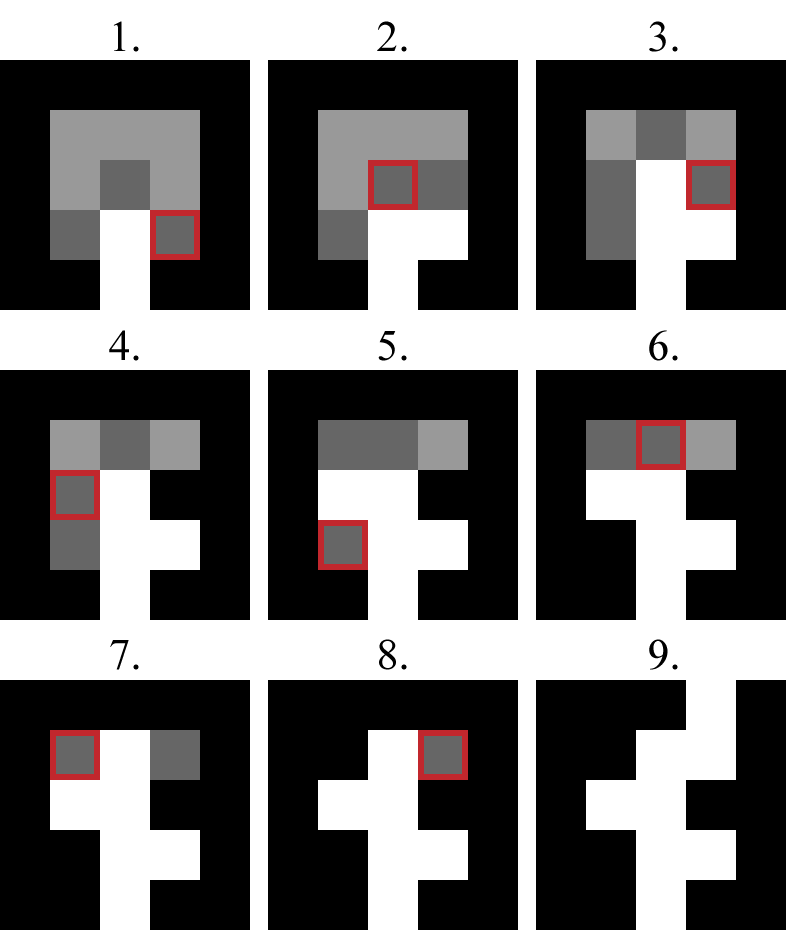
\includegraphics[width=0.45\textwidth]{../img/w09-lab/AlgorithmVisualized.png}
	\end{center}
	\caption{Visualisering av algoritmen när den genererar en labyrint av storleken 5x5.}
	\label{lab:maze:prims-algo-viz}
\end{figure}


\Task Gör färdigt den påbörjade algoritmen som skapar en slumpmässig labyrint enligt nedan.

\Subtask Inspektera ovanstående pseudokod och försök förstå den. Läs igenom uppgifterna nedan. Fråga om något är oklart.

\Subtask Studera de färdiga implementationerna av metoderna \texttt{addSurroundingWalls} och \texttt{isThreeWallsAround} och även den halvfärdiga metoden \texttt{random} i \texttt{Maze} i ditt workspace och se om du kan förstå vad de gör. Det underlättar stort om du kan skapa din egen mentala bild av hur algoritmen fungerar innan du börjar koda, t.ex. genom att rita exempel med papper och penna.

\Subtask Implementera metoden \texttt{random} i \texttt{Maze} som skapar och returnerar en slumpmässigt utformad labyrint med hjälp av pseudokoden ovan. Ta hjälp av metoderna \texttt{addSurroundingWalls} och \texttt{isThreeWallsAround}.

\Subtask Skapa en slumpmässig labyrint i ditt huvudprogram genom att anropa metoden \texttt{random}. Ett bra värde att använda när du anropar metoden är något tal mellan 20 och 100. Det vill säga anropa metoden genom att exempelvis skriva \texttt{random(50, 50)}. När du har slumpat fram en labyrint, testa att låta din sköldpadda gå igenom labyrinten och se om den lyckas!

\Subtask Om din algoritm har buggar, använd \code{println} för att instrumentera din kod, enligt tipsen som ges i appendix \ref{appendix:debug}, i arbetet med att åtgärda buggarna.

\begin{figure}[h]
	\begin{center}
		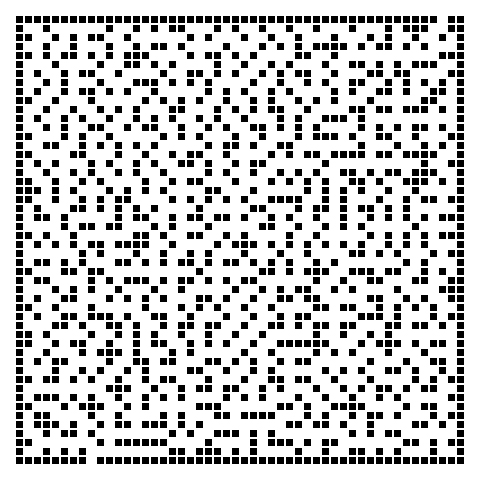
\includegraphics[width=1.0\textwidth]{../img/w09-lab/RandomMaze.jpg}
	\end{center}
	\caption{Ett exempel på hur en slumpmässigt utformad labyrint kan se ut.}
\end{figure}
